\section{Pipes and Filters}


Das Pipes and Filters Pattern (Pipeline und Filter Pattern?) stellt eine Struktur für Systeme zur verfügung, welche einen Datenstrom verarbeiten. Jeder Verarbeitungsschritt ist in einer Filter Komponente gekapselt. Daten werden über Pipes zwischen benachbarten Filtern ausgetauscht.

\subsection*{Example: Compiler}
 \textit{ASCII Quellcode -> [Lexical Analyzer] -> Token Stream -> [Syntax Analyzer] -> AST -> [Semantic Analyzer] -> ... -> Binaries}

\subsection*{Context}
Verarbeiten von Datenströmen (Processing data streams)

\subsection*{Problem}


Beim Entwickeln eines Systems welches einen Strom von Daten verarbeitet oder transformiert ist es nicht sinnvoll es als eine einzelne, grosse Komponente zu implementieren. Gründe dafür sind:

\begin{itemize}
	\item Entwicklung auf mehrere Entwickler aufteilen
	\item Die Art des Systems legt eine Aufteilung in verschiedene Verarbeitungsschritte nahe
	\item Die Anforderungen (Requirements) können sich noch ändern
\end{itemize}

Ob die Aufteilung in mehrere Verarbeitungsschritte sinnvoll ist, hängt stark von der Domäne und dem zu lösenden Problem ab. So können interaktive, ereignissgesteuerte Systeme nicht in Sequentielle Schritte unterteilt werden.

\subsubsection*{Forces}

\begin{itemize}
	\item Enhancements: Zukunftige Systemerweiterungen sollen durch das Austauschen von Verarbeitungsschritten oder neukombinieren von diesen (ggf auch durch den User) möglich sein.
	\item Reuse: Kleinere Verarbeitungsschritte können einfacher in einem anderen Kontext eingesetzt werden.
	\item Nicht benachbarte Verarbeitungsschritte tauschen keine Informationen aus
	\item Verschiedene Input Daten existieren, wie Netzwerk-Verbindungen oder Hardware-Sensoren.
	\item Ergebnisse sollen auf verschiedene Art und Weise präsentiert oder gespeichert werden
	\item Explizites Speichern von Zwischenresultaten für die weitere Verarbeitung in Dateien ist Fehleranfällig falls es durch den Benutzer gschieht.
	\item Man möchte parallele oder quasi-parallele Ausführung der Verarbeitungsschritte nicht ausschlissen.
\end{itemize}

\subsection*{Solution}


\begin{itemize}
	\item Aufteilen der Aufgabe in mehrere sequentielle Verarbeitungsschritte
	\item Schritte werden durch "Datenflüsse" verbunden (Output von Schritt N ist Input von Schritt N+1)
	\item Jeder Verarbeitungsschritt wird als "Filter" implementiert
	\begin{itemize}
		\item Filter sollten die Daten inkrementell verarbeiten (Es muss nicht aller Input entgegengenommen werden, bevor erster Output ausgegeben wird)
		\item Dadurch kann die Latenzzeit verringert werden und eine echt parallele Verarbeitung wird ermöglicht (Filter N und N+1 können parallel Arbeiten)
	\end{itemize}
	\item "Datenquelle" ist z.B. ein Textfile
	\item "Datensenke" ist ein Textfile, ein Terminal, eine Animationssoftware etc.
	\item Quelle, Filter und Senke werden durch "Pipes" verbunden
	\item * Pipes implementieren den Datenfluss zwischen benachbarten Schritten
	\item Eine Reihe von durch Pipes verbundene Filter wird "Processing Pipeline" genannt
\end{itemize}


Das Pipes and Filters Pattern unterteilt die Aufgabe des Systems in mehrere, sequenzielle Verarbeitungsschritte. Diese Schritte sind durch den Datenfluss verbunden, wobei die Ausgabe-Daten eines Schrittes die Eingabe-Daten des nächsten Schrittes sind. Jeder Verarbeitungsschritt ist durch eine Filter-Komponente implementiert. Diese Filter-Komponenten verarbeiten die Daten dabei inkrementel: laufend, Stück für Stück und nicht den Kompletten Input aufs mal, bevor die Daten weitergegeben werden. Dadurch wird die Latenz klein gehalten und parallele Verarbeitung ermöglicht. Die Daten kommen dabei von einer Daten-Quelle (z.B. eine Textdatei) über eine Pipe zum ersten Filtern und werden über weitere Pipes von Filter zu Filter weitergegeben, bis sie schliesslich nach dem letzte Filter über die letzte Pipe in einer Daten-Senke (z.B. auch ein Textfile) landen. Die Sequenz der durch Pipes verbundener Filter wird dabei "processing pipeline" genannt.

\subsection*{Structure}


\subsubsection*{Filter}


Es gibt drei verschiedene, grundlegende Arten wie ein Filter Input-Daten verarbeiten kann:

\begin{itemize}
	\item enrich (anreichen): Berechnen und Informationen hinzufügen
	\item refine (aufbereiten): Daten konzentrieren oder extrahieren
	\item transform (umwandeln): Daten in einer anderen Repräsentation ausgeben
\end{itemize}

Die Aktivität eines Filters kann auf verschiedene Arten ausgelöst werden:

\begin{itemize}
	\item Passiv: Das nachfolgende Pipeline-Element fordert Daten vom Filter an (pull)
	\item Passiv: Das vorhergehende Pipepline-Element reicht die Daten an den Filter weiter (push)
	\item Aktiv: Am Häufigsten: Der Filter ist in einer Schleife aktiv und fordert Daten an und gibt sie der Pipeline weiter (pull \& push)
	\item * Alle Unix Filter sind nach dieser Definition aktiv
\end{itemize}

Ein aktiver Filter startet die Verarbeitung selbst als separates Programm oder Thread.

Ein passiver Filter wird als Funktion (pull) oder prozedur (push) aufgerufen.

\subsubsection*{Pipes}


Pipes sind die Verbindungen zwischen Filtern und von der Daten-Quelle (data source) zu einem Filter, so wie von einem Filter zur Daten-Senke (data-sink). Falls zwei aktive Komponente verbunden werden kümmert sich die Pipe um die Synchronisation. Wird die Aktivität von einem der benachbarten Filter kontrolliert, kann die Pipe als direkter Aufruf der passiven Komponente durch die aktive Komponente implementiert werden. Allerdings machen direkte Aufrufe die Rekombination von Filtern schwieriger.

\subsubsection*{Data Source}


Die Datenquelle (data source) repräsentiert den Input des Systems und stellt eine Sequenz von Datenwerten des selben Typs dar.

Zum Beispiel:
\begin{itemize}
	\item Textdatei
	\item Sensor der ein Stream von Messdaten liefert
	\item Twitter Timeline
\end{itemize}

\subsubsection*{Data Sink}


Die Datensenke (data sink) sammelt die Resultate vom Ende der Pipeline. Eine aktive Datensenke fordert die Daten vom der vorhergegangen Verarbeitungsschritt an (pull), während eine passive Datensenke dem vorhergegangen Filter erlaubt die Daten in die Senke zu liefern oder zu schreiben.

Zum Beispiel:
\begin{itemize}
	\item Datei
	\item Visualisierung
	\item Konsolenoutput
\end{itemize}

\subsection*{Dynamics}

\begin{figure}[H]
	\centering
	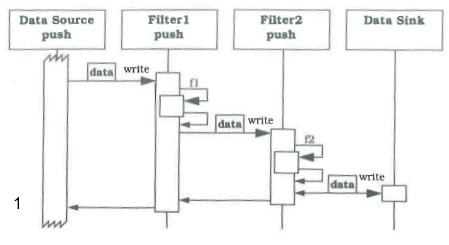
\includegraphics[width=0.7\textwidth]{content/posa1/images/pipes-and-filters-szen1.png}
	\caption{Pipes And Filters Szenario 1}
\end{figure}

\begin{figure}[H]
	\centering
	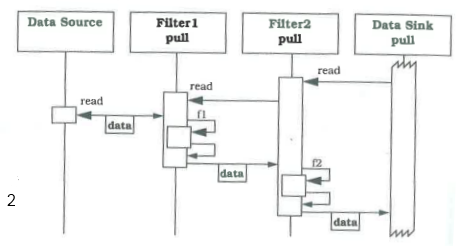
\includegraphics[width=0.7\textwidth]{content/posa1/images/pipes-and-filters-szen2.png}
	\caption{Pipes And Filters Szenario 2}
\end{figure}

\begin{figure}[H]
	\centering
	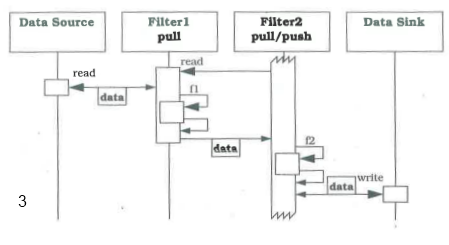
\includegraphics[width=0.7\textwidth]{content/posa1/images/pipes-and-filters-szen3.png}
	\caption{Pipes And Filters Szenario 3}
\end{figure}

\begin{figure}[H]
	\centering
	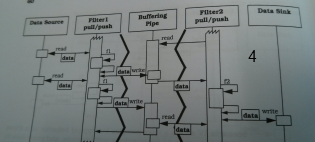
\includegraphics[width=0.7\textwidth]{content/posa1/images/pipes-and-filters-szen4.png}
	\caption{Pipes And Filters Szenario 4}
\end{figure}


\begin{enumerate}
	\item Push only, Datenfluss wird durch die Datenquelle gestartet und von Filter weitergegeben.
	\item Pull only, Datenfluss wird durch die Datensenke gestartet. Filter holen sich benötigte Daten.
	\item Ein Filter startet aktiv den Datenfluss und pullt die Daten vom vorherigen Filter / pusht die Daten zum nächsten Filter. Datenquelle und -senke sind passiv.
	\item Pipes werden als Buffer implementiert. Jeder Filter pullt Daten aus der vorherigen Pipe und pusht die Resultate in die nächste Pipe.
\end{enumerate}


\begin{enumerate}
	\item Unterteile das System in eine Sequenz von Verarbeitungsschritten, wobei jeder Schritt nur vom Output des direkten Vorgängers abhängig sein darf.
	\item Definiere ein Daten-Format welches durch die Pipes weitergegeben wird. Ein einheitliches Format stellt dabei die grösste Flexibilität sicher, da eine rekombinations der Filter einfach ist. Transformations-Filter ermöglichen dabei verschiedene Daten-Repräsentationen/-Formate.
	\item Entscheide wie jede Pipe-Verbindung implementiert werden soll. Dies bestimmt ob die Filter aktive oder passive Komponenten sein müssen.
	\item Entwirf und implementiere die Filter. Durch kleine, aktive Komponenten erreicht man eine hohe Flexibilität auf kosten von häufigen Kontextwechseln und Daten-Transfers.
	\item Entwirf die Fehlerbehandlung. Da Pipelines keinen gemeinsamen Zustand besitzen, kann die Fehlerbehandlung schwierig sein. Im Minimum sollte eine Fehlererkennung möglich sein. UNIX definiert einen speziellen Ausgabekanal für Fehler (stderr).
	\item Einrichten der Verarbeitungs Pipeline. Die kann bei einem einfachen Programm direkt in einer Main-Funktion erfolgen oder für eine grössere Flexibilität kann eine Shell oder ein User-Interface (grafisch) bereitgestellt werden.
\end{enumerate}


\subsubsection*{Tee and join pipeline systems}

\begin{itemize}
	\item Limitation von nur je einem Input und einem Output pro Filter kann aufgehoben werden
	\item Die Verarbeitung kann als gerichteter Graph dargestellt werden
	\item Dadurch werden auch Feedback Loops (Zyklen im Graph) ermöglicht
	\item * Achtung: Falls Zyklen vorhanden sind, muss sichergestellt werden, dass das System terminiert
	\item Restriktion auf azyklischen Datenfluss vereinfacht das System und ermöglicht trotzdem noch sehr nützliche Programme
\end{itemize}

\subsection*{Known uses}


\begin{itemize}
	\item UNIX (z.B. \textit{ls -s | sort -n}, stdout von ls wird zu stdin von sort weitergeleitet)
	\item CMS Pipelines (Erweiterung für das OS von IBM mainframes)
	\item LASSPTools (Toolset für numerische Analyse, bestehend aus Filterprogrammen die über UNIX Pipes verbunden werden können)
	\item LINQ Queries, Select(), Where(), GroupBy() etc. sind Filter die z.B. auf einer Liste angewendet werden. Die Filter werden erst angewendet, wenn das Resultat benötigt wird (Lazy Evaluation).
\end{itemize}

\subsection*{Consequences}


\subsubsection*{Benefits}


\begin{itemize}
	\item Keine Zwischendateien nötig (aber möglich)
	\item Flexiblität durch Austauschen von Filtern
	\item Flexiblität durch Neuanordnung von Filtern
	\item Wiederverwendung von Filter Komponenten
	\item Rapid-Prototyping von Pipelines (Lego System durch Verwendung von existierenden Filtern)
	\item Effizienz durch parallele Verarbeitung
\end{itemize}

\subsubsection*{Liabilities}


\begin{itemize}
	\item Austausch von Zustandsinformationen ist teuer oder inflexibel (z.B. Symbol Tabelle des Compilers wird von Lexer sowie von Parser benötigt)
	\item Effizenz Nutzen ist oft eine Illusion. (Die Kosten des Datentransfers zwischen Filtern kann höher sein als die eines Filters, einige Filter sammeln alle Eingabe-Daten bevor sie Daten ausgeben (z.B. bei Sortierung), Kontext-Wechsel ist teuer, Sychronisation)
	\item Daten-Transformations overhead. Nur ein Datentyp für alle Filter hat zwar die höchste Flexiblität, führt aber zu einem Overhead bei der Daten-Transformation.
	\item Fehlerbehandlung (error handling). Die Fehlerbehandlung ist die Achillesferse des Pipes and Filters pattern. Man sollte zumindest eine einfache Strategie für die Fehlerbenachrichtigung im System haben.
\end{itemize}

\subsection*{See Also}


\begin{itemize}
	\item Layers pattern
	\begin{itemize}
		\item Ist besser geeignet falls Fehler behandelt werden müssen
		\item Rekombination und Wiederverwendung ist aber nicht so einfach wie bei Pipes and Filters
	\end{itemize}
\end{itemize}

\subsection*{Mögliche Prüfungsfragen}


\begin{itemize}
	\item Weshalb sind Zyklen bei einem Tee and Join System so gefährlich?
\end{itemize}

